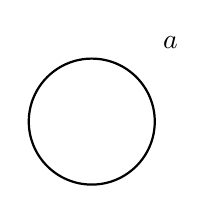
\begin{tikzpicture}[baseline=-0.2em, thick]
  \draw circle [radius=0.8] (0,0)
    (1,1) node {$a$};
\end{tikzpicture}
\! = d_a, \quad
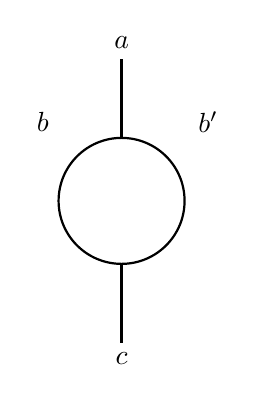
\begin{tikzpicture}[baseline=-0.2em, thick]
  \draw (0,1.8) node [above] {$a$} -- (0,-1.8) node [below] {$c$};
  \draw [fill=white] circle [radius=0.8] (0,0)
    (-1,1)  node {$b$}
    (1.1,1) node {$b'$};
\end{tikzpicture}
\!\! = \delta_{ac} \sqrt{\frac{d_b d_{b'}}{d_a}} \,
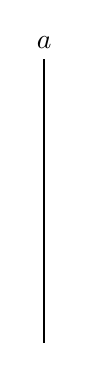
\begin{tikzpicture}[baseline=-0.2em, thick]
  \draw (0,1.8) node [above] {$a$} -- (0,-1.8);
\end{tikzpicture}
